\documentclass[10pt,letterpaper]{article}
\usepackage{tools}
\usepackage{enumitem}
%\settextfont{B Nazanin}
\usepackage{lipsum}
\setlength{\parskip}{3mm}
\setlength{\parindent}{0mm}
\newcommand{\wid}{0.49\textwidth}
\newcommand{\widone}{60mm}
\begin{document}
\Large
\begin{center}
In the name of beauty

6th problem set of ComNet course
\hl
\end{center}
Q1) Determine the following statements as true or false. (Use enough reasons and explanation to support your answer)

\begin{enumerate}[label=\alph*-]
\item
In TCP flow control mode, When the sender reads that the \texttt{rwnd} of the receiver is set to zero, it halts until the next ACK to arrive from receiver containing an updated \texttt{rwnd}.
\item
In 3-way handshaking, the SYN bit of all the first three packets exchanged between sender and receiver is set to 1. In turn, at the end of the connection, the client sends a segment with FIN bit set to 1 and deallocates the buffer.
\item
In an end-to-end congestion control paradigm, the Network Layer can assist the Transport Layer for declaring and feedbacking congestion.
\item
The sender can manipulate \texttt{cwnd} to trigger its sending rate in congestion control mechanism.
\item
Of the three components of congestion control (slow start, congestion avoidance, and fast recovery), only slow start and congestion avoidance are necessary.
\item
In fast recovery, the value of \texttt{cwnd} is increased by 1 MSS for every duplicate ACK received for the missing segment that caused TCP to enter the fast-recovery state.
\end{enumerate}

Q2) A TCP sender transmits 1500 bytes segments to a receiver. Assume that the segments arrive at the input of the receiver with buffer size = 6000 bytes at a bit rate of 12kbps. The Application Layer on the receiver side, however, is not ideal and will read the segments from the buffer at the speed of 6kbps. Consider time slots of 2 secs, starting from $t_0$ where the first bits of the first packet are accumulating in the buffer.
\begin{enumerate}[label=\alph*-]
\item
What is the value of \texttt{rwnd}, in bytes, that the receiver advertises to the sender at the end of the first time slot?
\item
At the end of which time slot does the receiver advertise \texttt{rwnd}=0 to the sender? What does the sender do in this case?
\end{enumerate}
(Reading packets by the App. Layer starts from the beginning of the buffer once at least a correct packet has been fully received.)

Q3)

Consider Figure 1. Assuming TCP Reno is the protocol experiencing the behavior shown above, answer the following questions. In all cases, you should provide a short discussion justifying your answer.
\begin{enumerate}[label=\alph*-]
\item
Identify the intervals of time when TCP slow start is operating.
\item
Identify the intervals of time when TCP congestion avoidance is
operating.
\item
After the 16th transmission round, is segment loss detected by a triple
duplicate ACK or by a timeout?
\item
After the 22nd transmission round, is segment loss detected by a triple
duplicate ACK or by a timeout?
\item
What is the initial value of ssthresh at the first transmission round?
\item
What is the value of ssthresh at the 18th transmission round?
\item
What is the value of ssthresh at the 24th transmission round?
\item
During what transmission round is the 70th segment sent?
\item
Assuming a packet loss is detected after the 26th round by the receipt of a
triple duplicate ACK, what will be the values of the congestion window
size and of ssthresh?
\item
Suppose TCP Tahoe is used (instead of TCP Reno), and assume that triple
duplicate ACKs are received at the 16th round. What are the ssthresh
and the congestion window size at the 19th round?
\item
Again suppose TCP Tahoe is used, and there is a timeout event at 22nd
round. How many packets have been sent out from 17th round till 22nd
round, inclusive?
\end{enumerate}

{\huge (Figure 1 on next page)}

\begin{figure}[htbp]
\centering
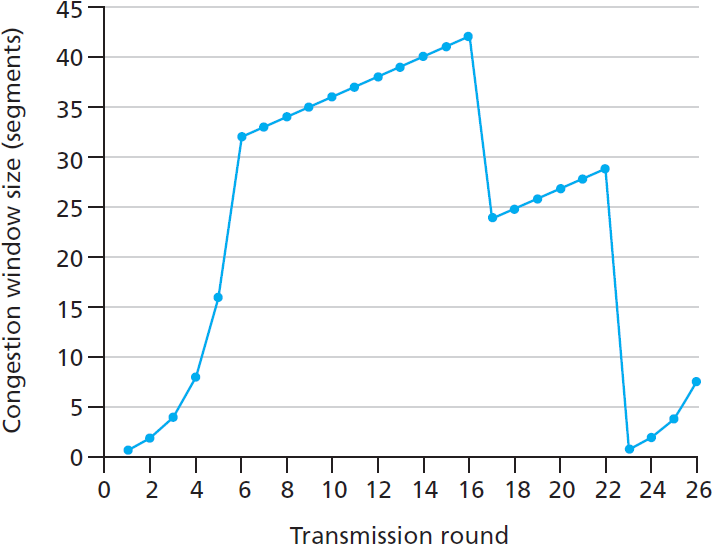
\includegraphics[width=150mm]{congestion.png}
\caption{TCP window size as a function of time}
\end{figure}
\end{document}